%
% 公立はこだて未来大学卒業研究中間報告書[全コース対応版]
%
%         ファイル名:"sample.tex"
%
%\documentclass[11pt]{jarticle}
\documentclass[11pt]{ujarticle} %%uplatexを用いる際はこちらを使用
\usepackage{funinfosys}
\usepackage{url}
\usepackage[dvipdfmx]{graphicx}
\author{%
b1017090 熊谷峻\\指導教員 : 松原克弥
}
\course{Information Systems Course}
%\course{Advanced ICT Course} %% 高度ICTコースの場合はこちらを使用
%\course{Information Design Course} %% 情報デザインコースの場合はこちらを使用
%\course{Complex Systems Course} %% 複雑系科学コースの場合はこちらを使用
%\course{Intelligent Systems Course} %% 知能システムコースの場合はこちらを使用
\title{VMMによる軽量かつセキュアなアドホッククラウド基盤}
\etitle{Lightweight and secure ad hoc cloud platform with VMM}
\eauthor{Shun Kumagai}
\abstract{近年,BYODやリモートワークの普及により,組織内に余剰な計算資源が散在するようになっている. そこで,この余剰計算資源を活用したクラウドコンピューティング技術である,アドホッククラウドが注目されている. これを取り入れることで,組織内の計算資源の利用率を向上させることができる. しかし,実行中のコードがPCに影響を与えたり,コード実行中のPCがクラウドから離脱することでクラウドジョブの持続が不可能になるといった課題が存在する. この課題に対処するために,本研究では,軽量なVMMであるBitVisorを用いてコードを実行するPCの環境を保護し,FaaS型クラウドを構築することでクラウドからの離脱を許容できるようなアドホッククラウド基盤を提案する.}
\keywords{VMM, アドホッククラウド, FaaS}
\eabstract{In recent years, due to the spread of BYOD and remote working, surplus computing resources are scattered throughout organizations. Therefore, ad hoc cloud computing technology, which is a cloud computing technology that makes use of these surplus computing resources, has been attracting attention. Ad-hoc cloud computing is one of the most popular cloud computing technologies. However, there are some problems, such as the impact of the running code on the PC and the persistence of the cloud job cannot be sustained due to the departure of the PC from the cloud. To deal with these problems, we propose an ad-hoc cloud infrastructure that protects the environment of the PC executing the code using BitVisor, a lightweight VMM, and allows the PC to leave the cloud by constructing a FaaS-type cloud. }
\ekeywords{VMM, ad hoc cloud, FaaS}
\begin{document}
\maketitle
%\vspace*{-.5cm}

\section{はじめに}
\subsection{背景}
近年,Bring Your Own Device (BYOD) の普及により,会社内に個人のPCを持ち込むことが増えている. そのため,業務を個人のPCで行うことは少なくない. また,リモートワークの増加により,会社に行かずに家で作業することが多くなっている. これら二つの要因により,組織内に利用されていないPCが増加している. これは言い換えると,組織内に余剰計算資源が散財していると言える.

この組織の余剰な計算資源を有効活用するため,次世代のクラウドコンピューティング環境としてアドホッククラウドが研究されている\cite{adhoc}. アドホッククラウドは,組織内で十分に活用されていない計算資源を利用して柔軟な計算インフラを作成することができる. また,余剰な計算資源を活用することで,組織内の計算資源の利用率を向上させることができるという利点がある.

\subsection{課題と目的}
アドホッククラウドを構築することで,組織内の余剰資源を活用することができるという利点がある一方で,3つの課題が存在する.

まず1つ目に,コードを実行するPCのユーザ環境に影響を及ぼすことがある. 例えば,実行中のコードによってPCの主プロセスを圧迫したり,クラッシュしてしまったりする可能性がある. そのため,ユーザ環境に影響を与えないようにセキュアにコードを実行しなければならない.

2つ目の課題として,異種OSプラットフォームへの対応がある. これはアドホッククラウドに参加する,組織内にある各PCのOSが異なる可能性があるためである. そのため,異種OSで実現可能なアーキテクチャが必要である.

3つ目の課題として,コード実行中のPCがクラウドから離脱してしまうという課題がある. これは,利用する計算資源がクラウド以外のタスクが増加することにより動的に変化することで起こる. そのため,実行中のPCがクラウドから離脱しても,他に実行中のコードやPCに影響を与えないクラウド環境が必要である.

そこで,本研究では,Virtual Machine Monitor(VMM) を用いたFaaS型クラウドを構築することで, 異種OSで実現可能な軽量かつセキュアなアドホッククラウドの仕組みの実現を目指す.

\section{既存技術}
\subsection{コンテナ}

1つ目の既存技術にコンテナがある.コンテナは,Linuxカーネル機能のcgroupやNamespaceを利用することで,CPUやメモリなどのリソースを隔離し,独立したOS環境を作り出すことができる技術である.Docker SwarmやKubernetesといったコンテナオーケストレーションツールを使って管理できる.これによって独立したコード実行環境の実現ができるため,セキュアなコード実行環境の実現ができる.

しかし,問題点として,コンテナの実現にLinuxカーネルの機能を使用しているため,Linux系OS以外では基本的に利用不可能である.仮想化を利用して,WindowsやmacOS上でLinux系OSを動作させることにより利用できるが,仮想化によるオーバーヘッドが増加してしまう.FaaS環境を構築できるOSS\cite{コンテナ}に,FissionやKubeless,OpenFaaS,OpenWhiskといったものがあるが,どのフレームワークもコンテナ技術をベースとしているため,異種OSに対応することができないという問題がある.

\begin{figure}[h]
  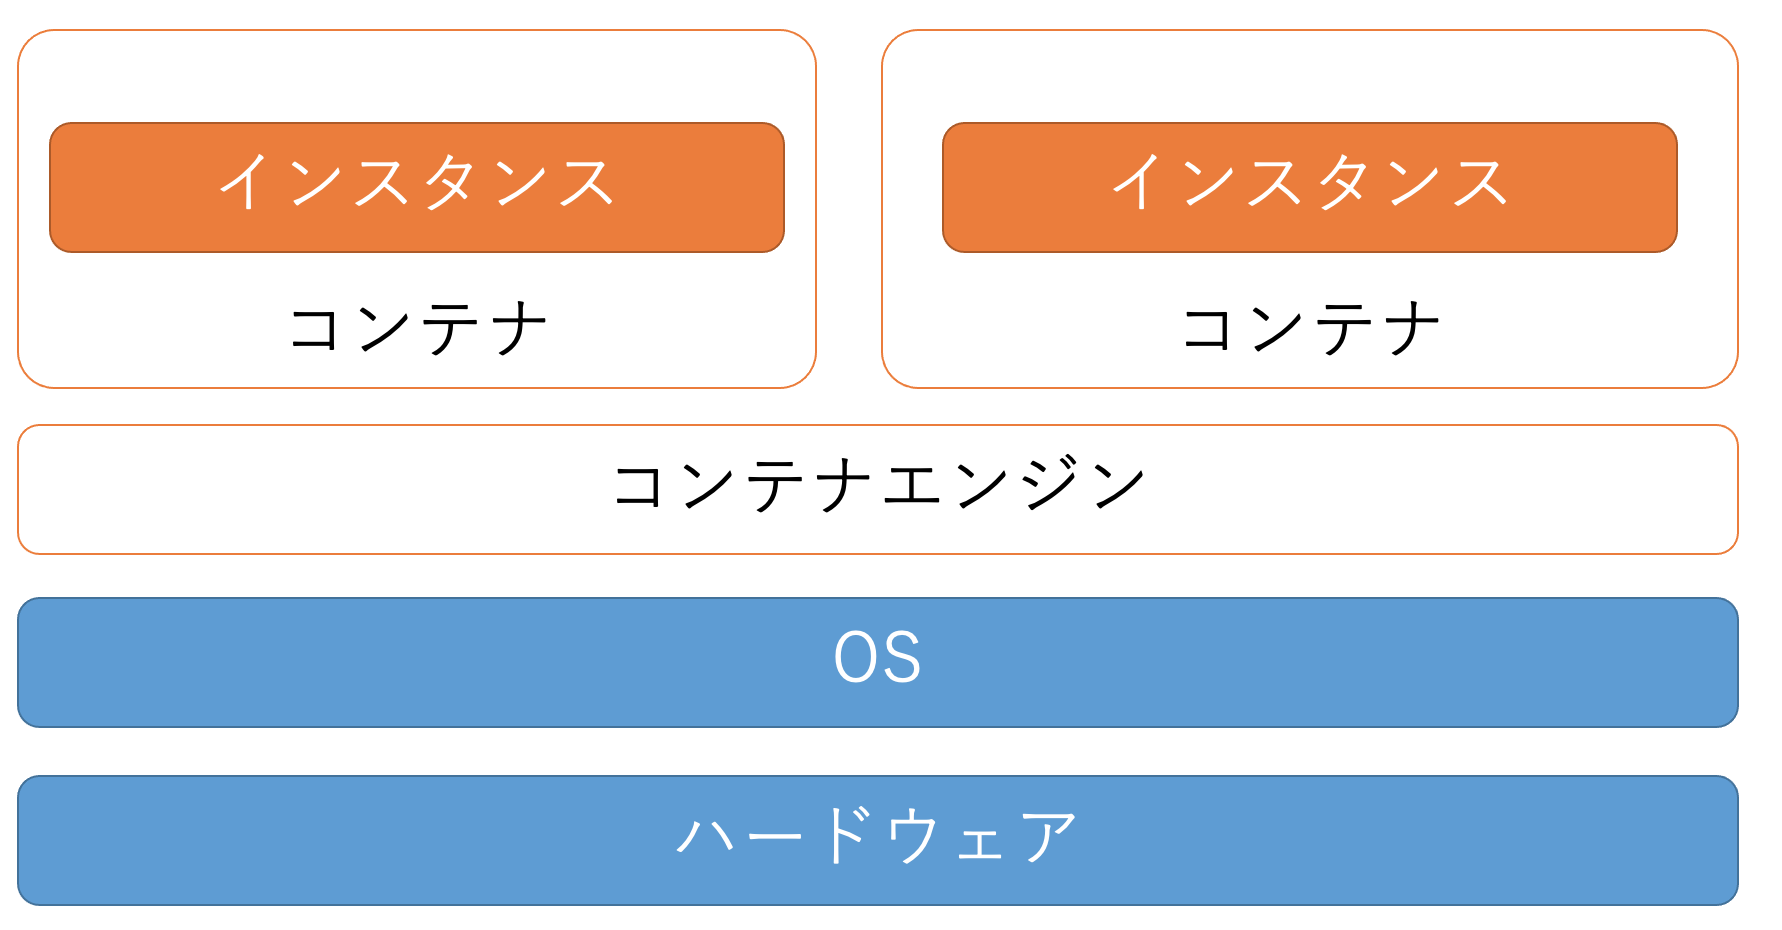
\includegraphics[width=8cm]{img/コンテナ.png}
\begin{center}図1 コンテナ\end{center}
\end{figure}

\subsection{プロセスマイグレーション}

2つ目の既存技術として,プロセスマイグレーションがある.プロセスマイグレーションとは別の環境にシステムやデータなどを切り替えることである.コードを実行中のインスタンスをマイグレーションすることにより,クラウドジョブを持続することができるため,コード実行中のPCがクラウドから離脱することを許容できるようになる.

しかし,問題点として,アドホッククラウドは動的に変化する計算資源を利用するため,頻繁にマイグレーションが発生してしまい,オーバーヘッドが発生することがある.また,異種OSで実現する場合は,複雑な実装と高度なマイグレーション方法が必要となってしまう\cite{プロセスマイグレーション}.

\begin{figure}[h]
  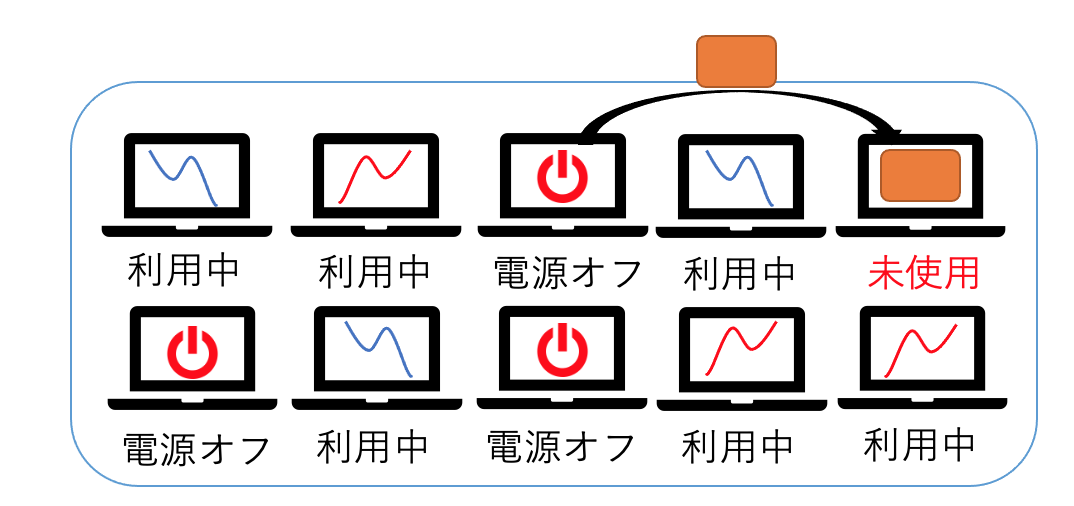
\includegraphics[width=8cm]{img/プロセスマイグレーション.png}
\begin{center}図2 プロセスマイグレーション\end{center}
\end{figure}

\section{先行研究}
\subsection{アドホッククラウドの先行研究}
アドホッククラウドの先行研究として,Garyらの研究がある\cite{gary}.Garyらはアドホッククラウドコンピューティングプラットフォームを提案している.計算機を利用できる時間が散発的になるような信頼性の低いインフラ上で動作する場合でも,アドホッククラウドはクラウドジョブを正常に完了できる信頼性の高いプラットフォームであることが示された.

しかし,仮想化の仕方や利用するVMMによっては,仮想化によるオーバーヘッドが大きくなってしまうことが示唆されている.

\subsection{BitVisorの先行研究}
BitVisorを利用した先行研究として,芹川らの研究がある\cite{ボランティア}.芹川らは, BitVisorを用いて,ボランティアコンピューティングにおける組織側の計算内容の保護及びボランティア側のマシン環境の保護を行うことで,双方のセキュリティを強化する方法を提案した.ボランティアコンピューティングは,分散コンピューティングの一つであり,管理サーバから送られた計算コードを個人のPC上で実行し,その結果をサーバに送り返すものである.個人のPCの余剰計算資源を有効活用するという点が,アドホッククラウドと共通の概念である.研究の結果,セキュアにボランティアコンピューティングを行うことができる仕組みを実現した.

しかし,この手法はあくまでもボランティアコンピューティングに向けた仕組みであるため,アドホッククラウドに応用する場合,計算結果を管理サーバにではなく,ユーザに送信しなければならない.また,利用可能な計算資源が変化することで起こるクラウドからの離脱を考慮する必要がある.

\subsection{提案}
本研究では,Function as a Service(FaaS) 型クラウドを構築し,軽量なVMMであるBitVisorを用いたセキュアなアドホッククラウド基盤を提案する.提案の図は以下のようになっている.

\begin{figure}[h]
  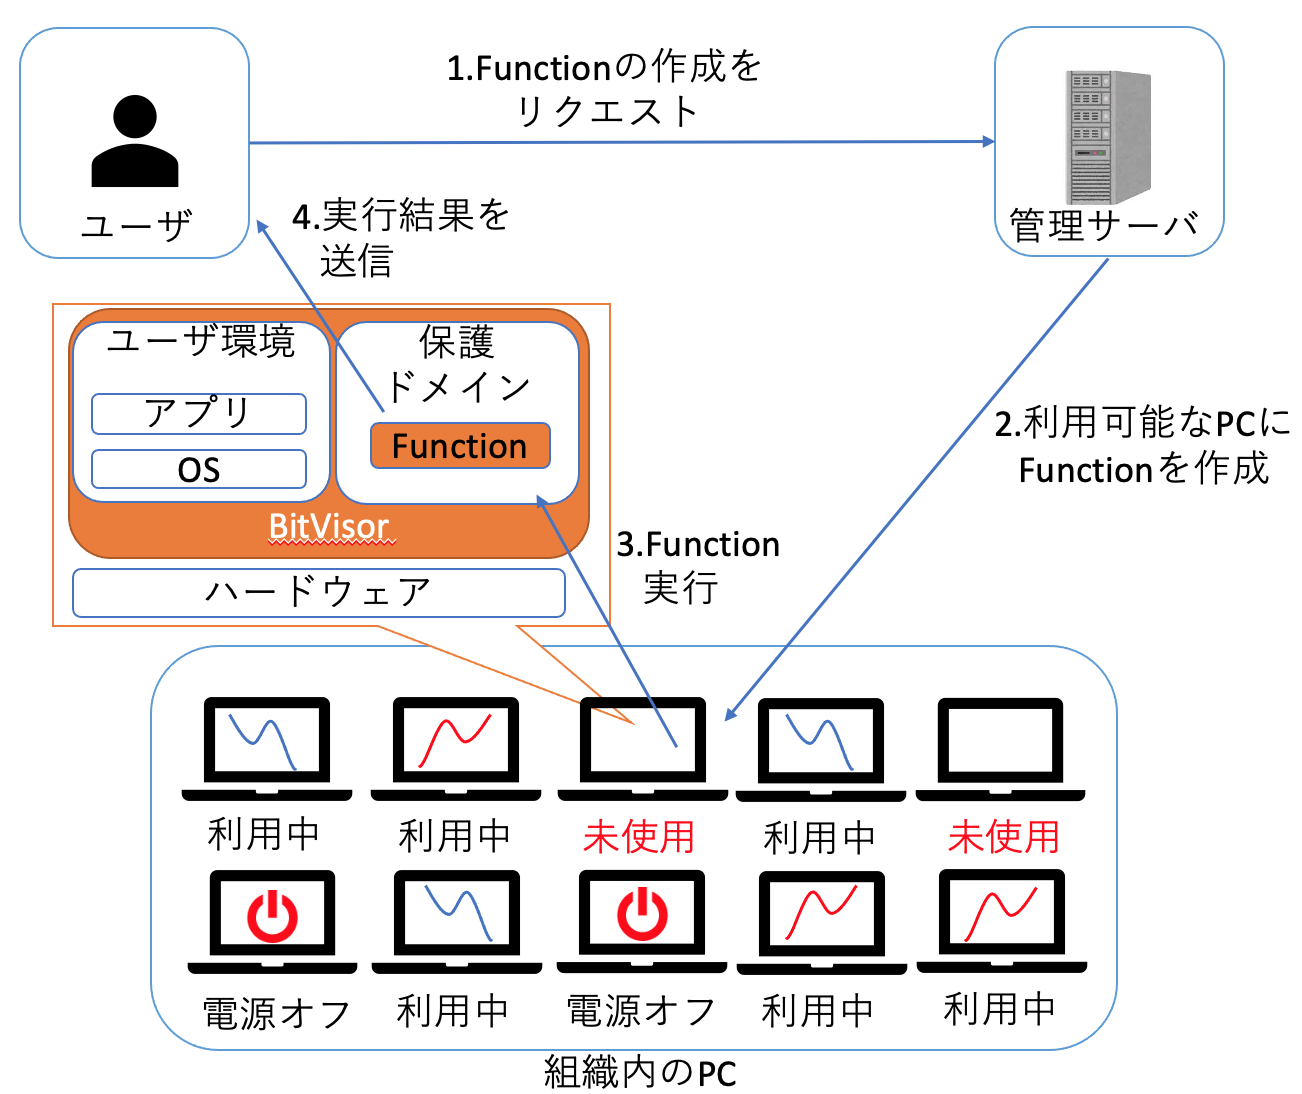
\includegraphics[width=8cm]{img/提案図.png}
\begin{center}図3 提案図\end{center}
\end{figure}

\subsection{FaaS}
クラウドサービスにはいくつかの種類があり,Infrastructure as a Service (IaaS)や,Platform as a Service (PaaS),Software as a Service (SaaS)などがある\cite{cloud1}\cite{cloud2}.しかし,これらのクラウドサービスは,ステートフルなシステムであるため,利用中のサーバがクラウドから離脱してしまった場合,クラウドを持続するために高速なマイグレーションが必要となる.

そこで,この問題を回避するために,本研究ではFaaS型クラウドを構築する.FaaSは,サーバレスアーキテクチャを実現する手法の一つで,Functionという単位で処理を実行できるクラウドサービスである.リクエストに応じてFunctionを実行するイベントドリブンという機能や,Functionの実行状態やマシンの情報を保持せず,入力された内容から一意に結果が決まるステートレスという特徴をもっている.これにより,Function実行中のPCが急にクラウドから離脱することがあっても,他のPCやFunctionに影響を与えることを防ぐことができるため,クラウドから離脱することを許容できるようになる.

\subsection{Virtual Machine Monitor(VMM)}
\begin{figure}[h]
  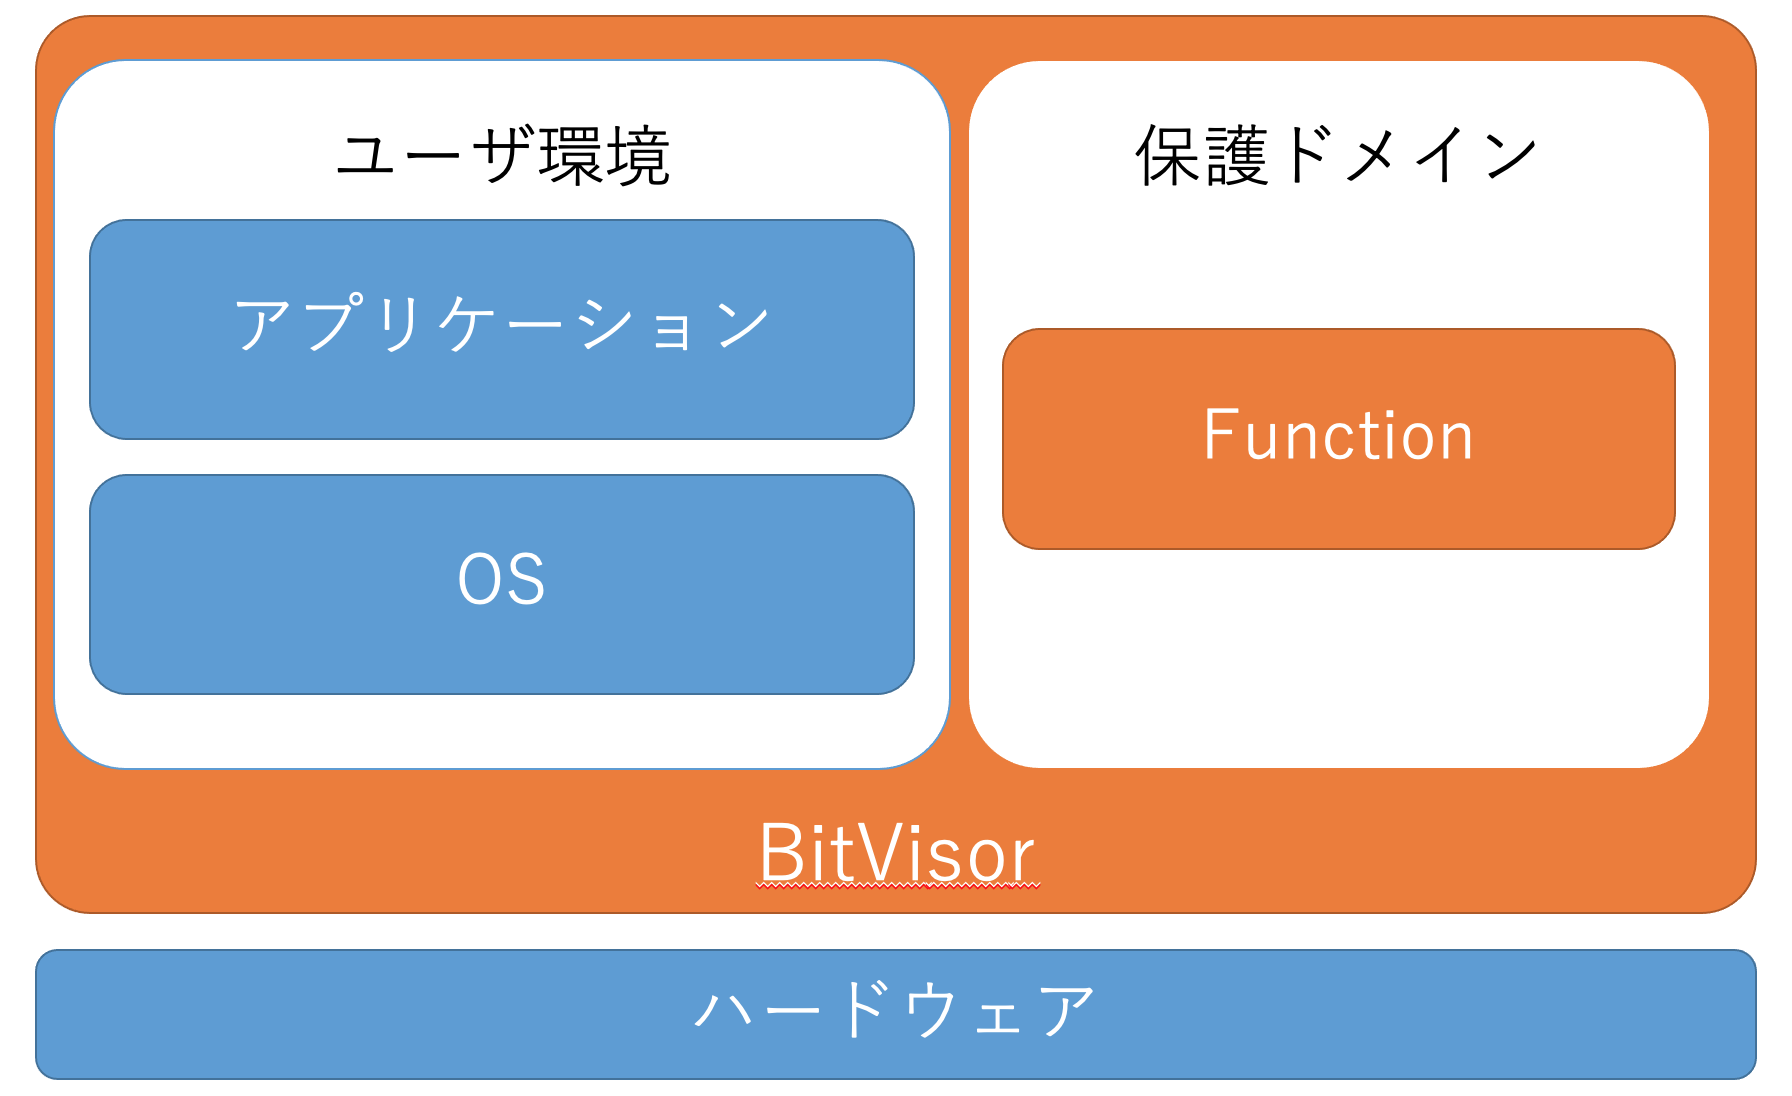
\includegraphics[width=8cm]{img/BitVisor.png}
\begin{center}図4 BitVisorと保護ドメイン\end{center}
\end{figure}
本研究では,VMMを利用する.VMMはハイパーバイザとも呼ばれる,ハードウェアとOSの間で動作するソフトウェアである.ホストOS上で動作するホスト型と違って,ハイパーバイザ型は,OSよりも下の層に位置するため,ハードウェアへアクセスする際にホストOSを経由しない.そのため,仮想化によるオーバーヘッドを抑えることができ,OSに依存しないので異種OSで実現可能となる. しかし,OSとハードウェアの通信にVMMが介在することによってオーバーヘッドが発生してしまう.そこで,軽量なVMMであるBitVisorを活用する\cite{BitVisor}.

BitVisorは,特定のデバイスのみ仮想化し,必要最低限のI/Oのみを監視・制御する準パススルー型VMMである.また,本来ハイパーバイザは複数のゲストOSで動作するが,その機能が省略されているため,軽量なことが特徴である.このBitVisorを利用することで,仮想化によるオーバーヘッドを軽減する.さらに,BitVisorには,計算資源は共有しつつも,ユーザ環境から隔離された実行環境を実現できる保護ドメインという機能がある.この保護ドメインにFunctionを作成することで,ユーザ環境へ影響を与えることを防ぐ.


\section{まとめ}
本研究の背景には,BYODやリモートワークの増加によって組織内に余剰な計算資源が散在しており,この余剰計算資源を活用することができるアドホッククラウドコンピューティングが注目されていることがある.しかし,アドホッククラウドを実現するにあたって,コードを実行するPCのユーザ環境に影響を及ぼす可能性がある,異種OSプラットフォームへの対応,コード実行中のPCがクラウドから離脱する可能性があるという3つの課題がある.そこで,本研究で提案するのが,軽量なVMMであるBitVisorを用いたFaaS型アドホッククラウド基盤である.ステートレスという特徴をもつFaaS型のクラウド環境を構築することで,クラウドからの離脱を許容できるようになる.さらに,BitVisorを活用することで,仮想化によるオーバヘッドを軽減し,異種OSで実現可能となる.また,保護ドメイン内にFunctionを作成することで,ユーザ環境を保護する.これによって,軽量かつセキュアなアドホッククラウド基盤を実現する.

\section{情報システムコースにおける本研究の位置づけ}
本研究では、安心・安全・快適な情報社会を支援する観点から、価値ある情報システムの創造、効率性と信頼性を考慮した情報システムの実現、多様で大規模な情報の生成と分析に関する具体的な課題に取り組み、その結果の評価を通じて、新しい方法論や、学問領域を切り拓く能力を育むことをカリキュラムポリシーとして掲げている.

本研究では,VMMを用いてアドホッククラウドコンピューティングについての課題に取り組むという,効率性と信頼性を考慮した情報システムの実現を目指している.
今後は実装を行い,デプロイしたFunctionを保護ドメインを通して実行できるかや,Function実行中にクラウドから離脱した場合,他のFunctionへの影響を防げるか評価を行う.

\begin{thebibliography}{99}
\bibitem{adhoc}
B. Varghese et al.,Next generation cloud computing: New trends and research directions,Future Generation Computer Systems,79,849–861,2018.
\bibitem{コンテナ}
Mohanty et al.,An Evaluation of Open Source Serverless Computing Frameworks,CloudCom,115-120,2018.
\bibitem{プロセスマイグレーション}
松原克弥,永井陽太,散在する余剰計算資源を活用したアドホッククラウド・システムの実現手法,IA2019-Workshop on Internet Architecture and Applications 2019,119,73–78,2019.
\bibitem{gary}
McGilvary et al.,Ad hoc cloud computing,2015 IEEE 8th International Conference on Cloud Computing,1063-1068,2015.
\bibitem{ボランティア}
芹川大地 et al.,Vmmによる軽量かつセキュアなボランティアコンピューティング基盤の実現,研究報告システムソフトウェアとオペレーティング・システム (OS),14,1–7,2012.
\bibitem{cloud1}
Dillon,Tharam and Wu,Chen and Chang,Elizabeth,Cloud computing: issues and challenges,2010 24th IEEE international conference on advanced information networking and applications,27-33,2010.
\bibitem{cloud2}
Xu,Xun,From cloud computing to cloud manufacturing,Robotics and computer-integrated manufacturing,28,75-86,2012.
\bibitem{BitVisor}
保理江高志 et al.,仮想マシンモニタbitvisorとi/o仮想化技術,情報処理学会研究報告システムソフトウェアとオペレーティング・システム(OS),2009,35–41,2009.
\end{thebibliography}
\end{document}
%
%
% EOF
